\documentclass[12pt, a4paper]{article}

% --- Paquetes ---
\usepackage[utf8]{inputenc}
\usepackage[spanish, es-tabla]{babel}
\usepackage{graphicx}
\usepackage{amsmath}
\usepackage{amsfonts}
\usepackage{amssymb}
\usepackage{tikz}
\usepackage{geometry}
\usepackage{xcolor}
\usepackage{listings}
\usepackage{hyperref}

\geometry{margin=2.5cm}
\usetikzlibrary{shapes.geometric, arrows, positioning, boxen}

% --- Estilos ---
\tikzstyle{block} = [rectangle, draw, fill=blue!10, text width=6em, text centered, rounded corners, minimum height=3em, font=\small]
\tikzstyle{io} = [trapezium, trapezium left angle=70, trapezium right angle=110, draw, fill=green!10, text width=4em, text centered, font=\small]
\tikzstyle{line} = [draw, -latex', thick]

\title{Marco Experimental: Diseño e Implementación de un Sistema de Videojuego Pong (Futbolito) en FPGA}
\author{Proyecto de Arquitectura de Computadoras}
\date{\today}

\begin{document}

\maketitle

\section{Introducción}
El presente marco experimental describe el entorno, las herramientas y la metodología utilizada para la implementación de un videojuego tipo Pong, denominado "Futbolito", sobre hardware reconfigurable. El diseño se centra en la generación de señales de video VGA y la gestión de lógica de juego en tiempo real mediante el lenguaje de descripción de hardware VHDL.

\section{Equipamiento y Materiales}
Para el desarrollo y validación del sistema, se utilizaron los siguientes recursos:

\subsection{Hardware}
\begin{itemize}
    \item \textbf{Tarjeta de Desarrollo:} Terasic DE2-115, la cual integra una FPGA Altera/Intel Cyclone IV E (modelo \texttt{EP4CE115F29C7}).
    \item \textbf{Puerto VGA:} Conector DB15 integrado en la placa con convertidores DAC de 8 bits por canal.
    \item \textbf{Monitor:} Pantalla compatible con el estándar VGA con resolución de al menos 640x480 píxeles.
    \item \textbf{Periféricos de Entrada:} Pulsadores (Pushbuttons) integrados para el control de los jugadores.
\end{itemize}

\subsection{Software}
\begin{itemize}
    \item \textbf{Quartus Prime Lite Edition:} Utilizado para la síntesis, asignación de pines y programación de la FPGA.
    \item \textbf{ModelSim Altera:} Empleado para la simulación funcional de los módulos de sincronización y lógica.
    \item \textbf{Python 3:} Uso de scripts (\texttt{img\_to\_vhdl.py}) para la conversión de imágenes de mapa de bits a archivos de inicialización de memoria (ROM) en VHDL.
\end{itemize}

\section{Configuración del Sistema}

\subsection{Arquitectura General}
El sistema se organiza en una estructura jerárquica modular, donde un módulo de alto nivel (\texttt{top\_futbolito}) interconecta los bloques funcionales principales. 

\begin{center}
    \begin{tikzpicture}[node distance = 2.5cm, auto]
        % Nodos
        \node [block] (clk) {Oscilador 50\,MHz};
        \node [block, right of=clk, node distance=3.5cm] (pll) {Video PLL (25.175\,MHz)};
        \node [block, below of=pll, node distance=2.5cm] (top) {Top Entity (VGA\_BALL)};
        \node [block, left of=top, node distance=3.5cm] (sync) {Controlador VGA (vga\_sync)};
        \node [block, right of=top, node distance=3.5cm] (logic) {Lógica de Juego (BALL)};
        \node [block, below of=logic, node distance=2cm] (rom) {Ball ROM (Sprite)};
        \node [io, below of=sync, node distance=2cm] (vga_out) {Monitor VGA};
        
        % Líneas
        \path [line] (clk) -- (pll);
        \path [line] (pll) -- (top);
        \path [line] (top) -- (sync);
        \path [line] (top) -- (logic);
        \path [line] (sync) -- (vga_out);
        \path [line] (rom) -- (logic);
        \path [line] (logic.west) -- (sync.east);
    \end{tikzpicture}
\end{center}

\subsection{Asignación de Pines (Pinout)}
La siguiente tabla resume las conexiones físicas más relevantes configuradas en el archivo \texttt{.qsf}:

\begin{table}[h]
    \centering
    \begin{tabular}{|l|c|l|}
        \hline
        \textbf{Señal de Diseño} & \textbf{Pin FPGA} & \textbf{Descripción} \\ \hline
        \texttt{Clock\_50Mhz} & PIN\_Y2 & Reloj maestro del sistema. \\ \hline
        \texttt{VGA\_Red[7..0]} & H10 a E12 & Bus de color Rojo (8 bits). \\ \hline
        \texttt{VGA\_Green[7..0]} & G8 a C9 & Bus de color Verde (8 bits). \\ \hline
        \texttt{VGA\_Blue[7..0]} & B10 a D12 & Bus de color Azul (8 bits). \\ \hline
        \texttt{VGA\_HSync} & PIN\_G13 & Sincronía Horizontal. \\ \hline
        \texttt{VGA\_VSync} & PIN\_C13 & Sincronía Vertical. \\ \hline
        \texttt{BTN\_UP\_LEFT} & PIN\_R24 & Control jugador izquierdo (Arriba). \\ \hline
        \texttt{BTN\_DOWN_LEFT} & PIN\_M23 & Control jugador izquierdo (Abajo). \\ \hline
    \end{tabular}
    \caption{Asignación de pines en la DE2-115.}
\end{table}

\section{Desarrollo Experimental}

\subsection{Generación de Video VGA}
Se implementó un estándar de 640x480 píxeles a una frecuencia de refresco de 60\,Hz. Los parámetros de temporización definidos en el módulo \texttt{vga\_sync.vhd} son:
\begin{itemize}
    \item \textbf{Pixel Clock:} 25.175 MHz.
    \item \textbf{Horizontal:} 640 activos, total 800 (Front Porch, Sync Pulse, Back Porch).
    \item \textbf{Vertical:} 480 activos, total 525 líneas.
\end{itemize}

\subsection{Lógica de Movimiento y Colisión}
El módulo \texttt{BALL.VHD} gestiona la posición del balón $(X, Y)$ y la lógica de colisiones. La actualización ocurre durante el intervalo del Vertical Retrace para evitar parpadeos (\textit{tearing}).
\begin{equation}
    \text{Posicion}_{n+1} = \text{Posicion}_{n} + \text{Motion}
\end{equation}
Se implementó una detección de bordes y colisión con las "raquetas" (paddles) invirtiendo el vector de movimiento al detectar coincidencia de coordenadas.

\section{Resultados Obtenidos}
La implementación exitosa del sistema permitió visualizar gráficos fluidos y una respuesta inmediata a los controles físicos. En la Figura \ref{fig:mockup} se observa una representación conceptual del sistema en funcionamiento.

\begin{figure}[h]
    \centering
    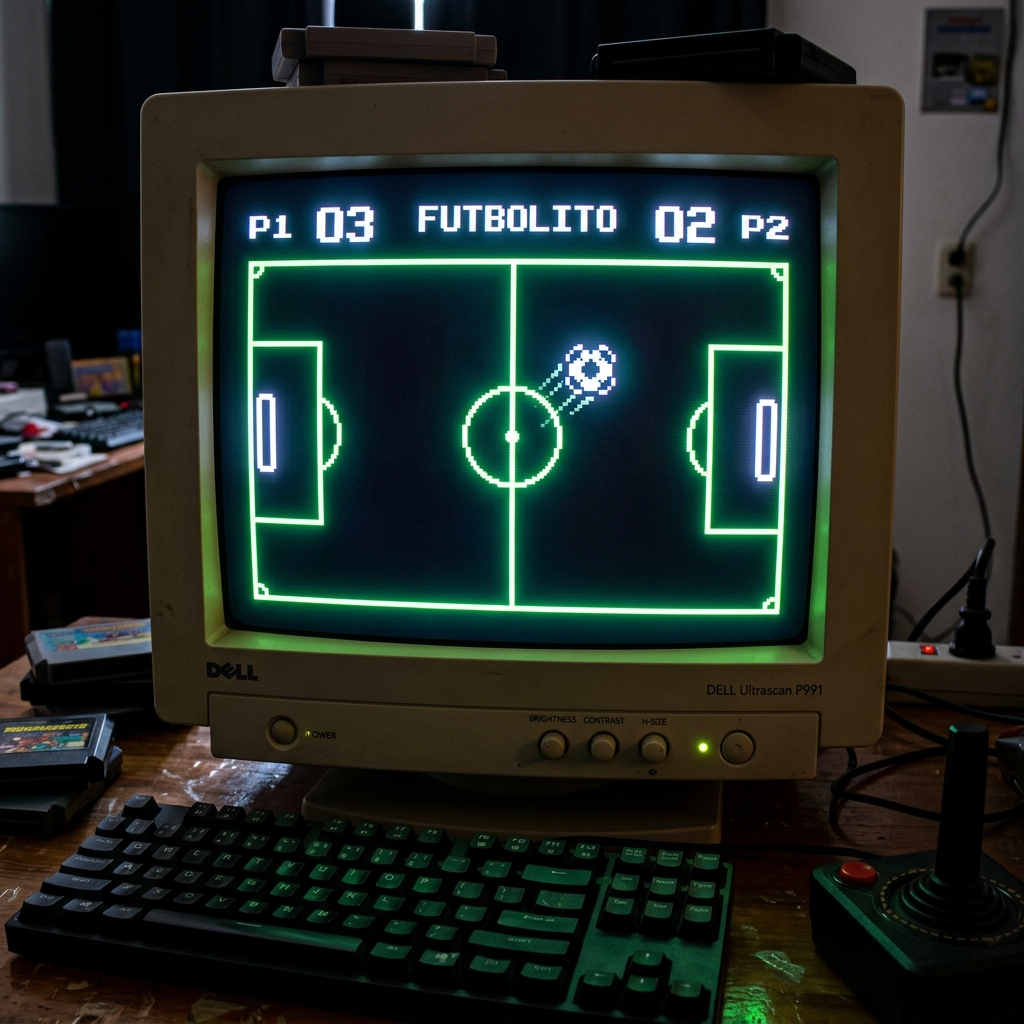
\includegraphics[width=0.7\textwidth]{assets/pong_vga_mockup.png}
    \caption{Representación conceptual del juego Futbolito sobre salida VGA.}
    \label{fig:mockup}
\end{figure}

\section{Conclusiones}
El marco experimental demuestra la viabilidad de utilizar FPGAs para el procesamiento de gráficos en tiempo real sin dependencia de procesadores de propósito general. La arquitectura modular permitió una depuración eficiente y una escalabilidad adecuada para futuras mejoras.

\end{document}
